\documentclass[oneside]{book}
\usepackage{glossaries}
\usepackage{derivative}
\usepackage{pgfplots}
\usepackage{graphicx}
\usepackage{tikz}
\usepackage{float}
\usepackage{booktabs}
\usepackage{circuitikz}
\usepackage{amsmath}
\usepackage{fancyhdr}
\usepackage{amssymb}
\usepackage[list=true]{subcaption}
\usepackage{lastpage}
\usepackage{array}
\usepackage[hidelinks]{hyperref}
\usepackage[a4paper,
    left=10mm,
    right=10mm,
    top=12mm,
    bottom=12mm,
]{geometry}
\setcounter{tocdepth}{3}
\newcolumntype{P}[1]{>{\centering\arraybackslash}p{#1}}
\begin{document}
\pagestyle{fancy}
    \fancyhf{}
\fancyhead[L]{EGB120 Foundations of Electrical Engineering}
\fancyhead[R]{\nouppercase{\leftmark}}
\fancyfoot[L]{Dinal Atapattu}
\renewcommand{\footrulewidth}{0.4pt}
\fancyfoot[R]{Page \thepage\ of \pageref{LastPage}}
    \title{
            Queensland University of Technology\\
            \rule{\linewidth}{0.5pt}
        \centering
        \textbf{EGB120} \\
        Tutorial Answers\\
        \vspace{0.4cm}
        \rule{\linewidth}{1.5pt}
        \small{\textit{Professor Geoff Walker}}
    }
    \author{Dinal Atapattu}
    \date{\today}
    \maketitle
    \thispagestyle{empty}
    \tableofcontents
        \section{Tutorial 7 \- Sequential Switching}
Consider the circuit below. The initial current in the inductor is $i_l(0-) = 0$. Find expressions for
$iL(t)$ and $v(t)$ for $t \geq 0$ and sketch to scale versus time.
\begin{figure}[H]
    \centering
    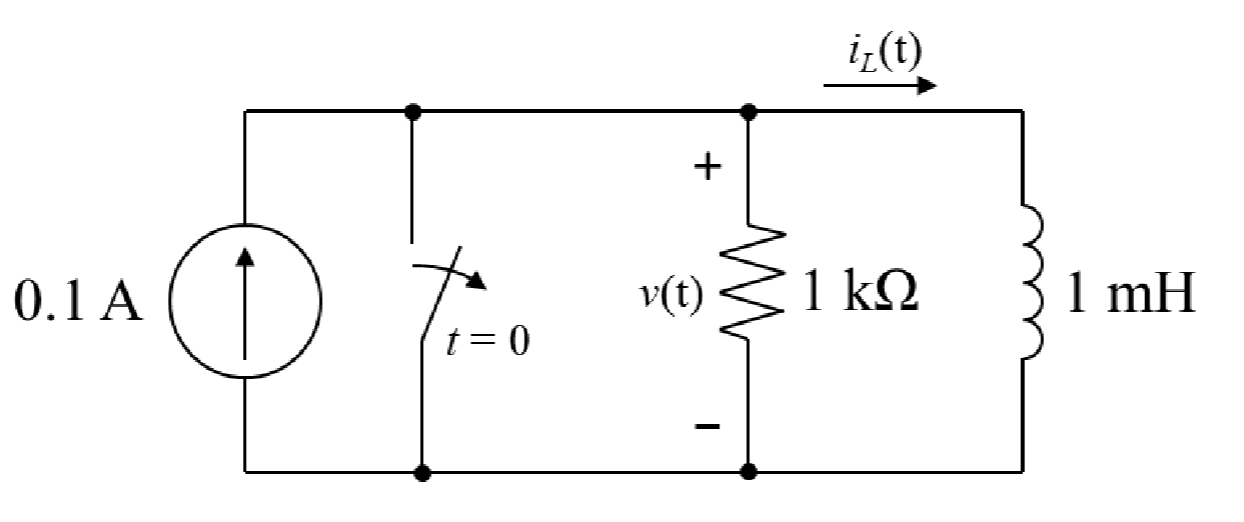
\includegraphics[width=0.4\linewidth]{tutorials/figures/seq_switch_practice.png}
\end{figure}
The given circuit is an RL circuit, therefore, step response is given by
\begin{equation*}
    i(t) = \frac{V_s}{R} + \left(I_0 - \frac{V_s}{R}\right)e^{-\frac{R}{L}t}
\end{equation*}
By applying a source transformation (Norton equivalent to Thevenin equivalent) we get
\begin{align*}
    V_s &= I_s R = 0.1 \times 1 \times 10^3 = 0.1 \times 10^3 V = 100V\\
\end{align*}
Using this we get that
\begin{align*}
    i(t) &= \frac{100}{1000} + \left(0 - \frac{100}{1000}\right)e^{-\frac{1000}{1\times{-3}}t} &&= 0.1 - 0.1e^{-1\times10^6 t} \\
    v(t) &= L \odv{i}{t} = 1\times10^{-3} \times \odv{}{t} \left(0.1 - 0.1e^{-1\times10^6 t}\right) = 0.1\times10^3 e^{-1\times10^6 t} &&= 100e^{-1\times10^6 t}
\end{align*}
\subsection{Tutorial Question}
    Igor the Mad Scientist is planning to reanimate a corpse (again). His plan is to capture energy
    from a lightning bolt into a capacitor, and then to discharge the capacitor into the torso and
    brain. The lower body is reanimated from a voltage supply. The electrical models of the body
    parts are shown in the figure below
    \begin{figure}[H]
        \centering
        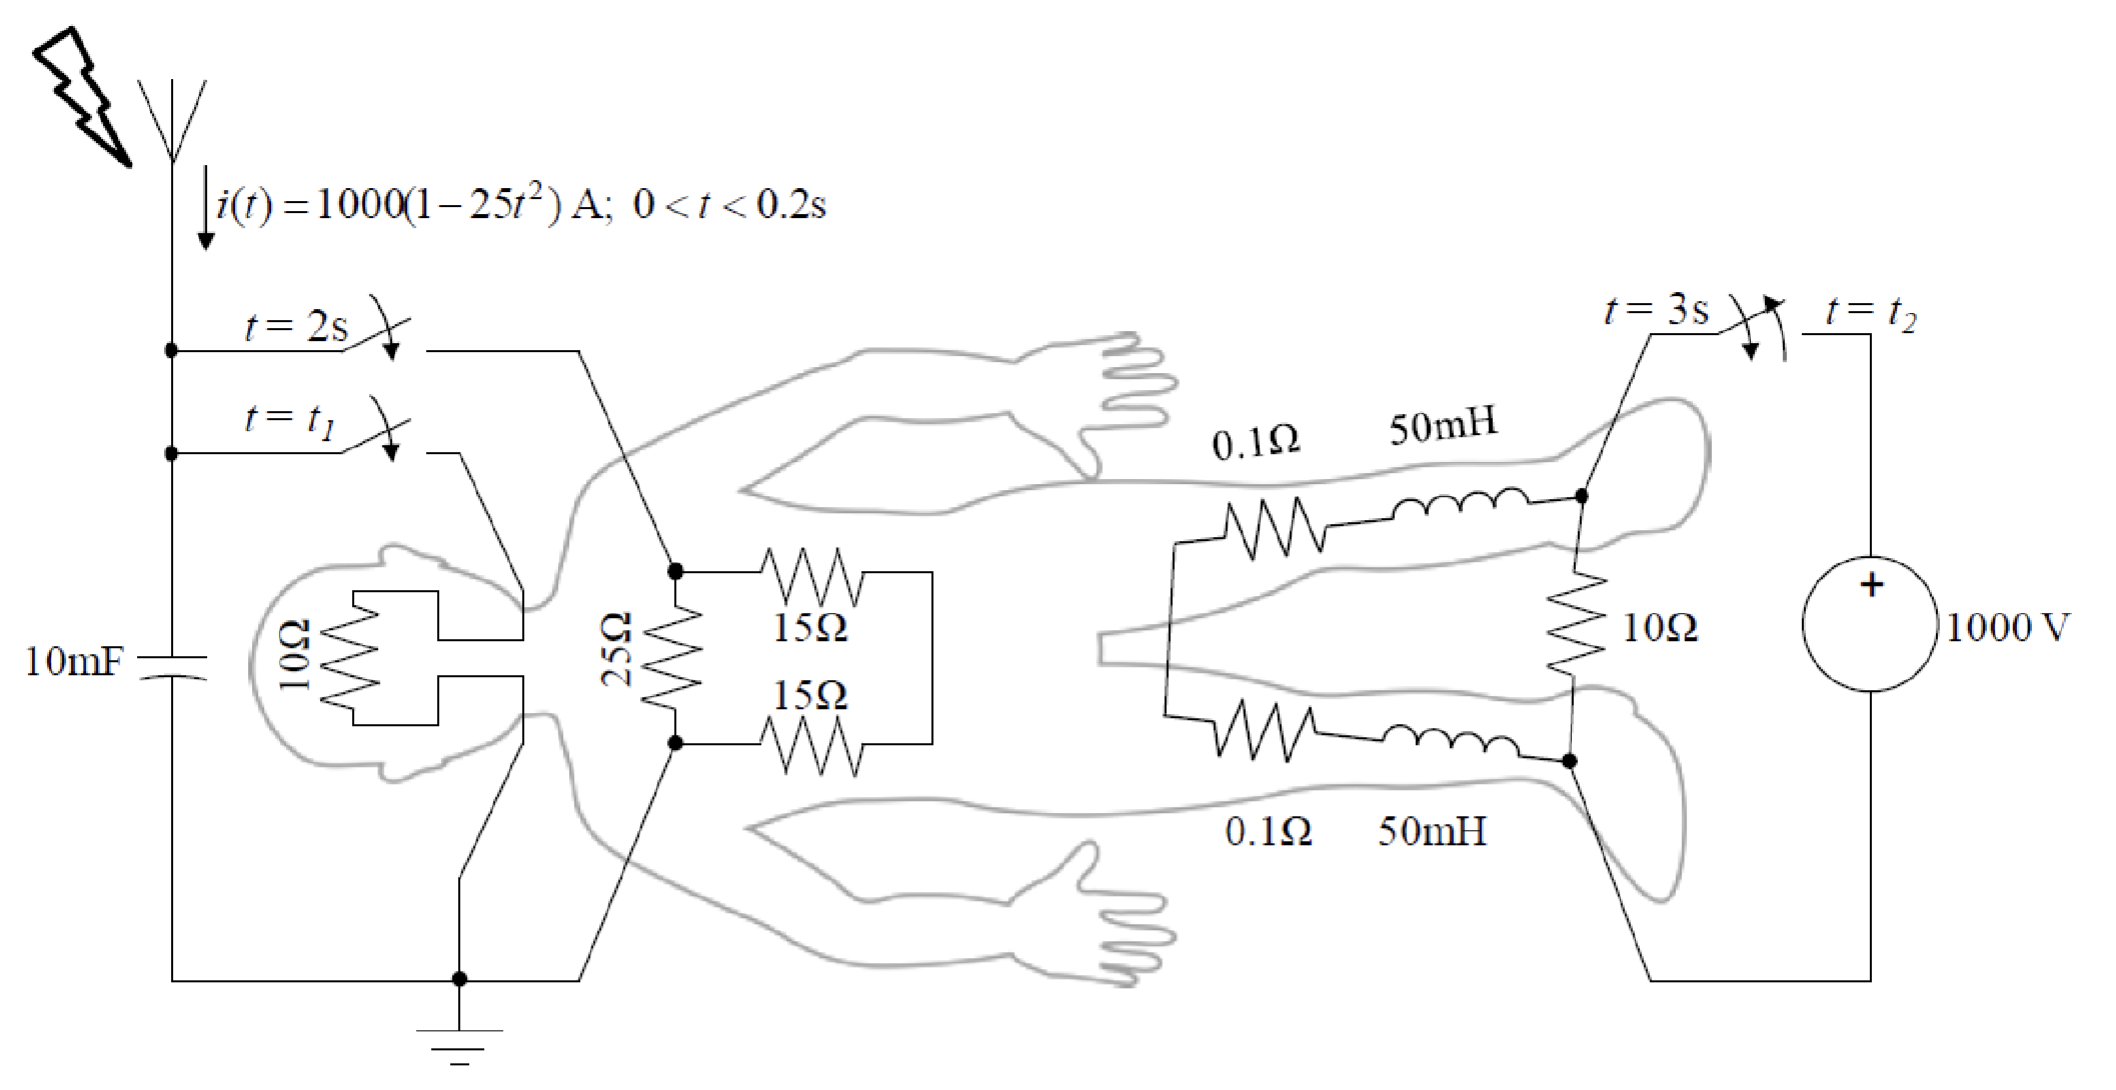
\includegraphics[width=0.6\linewidth]{tutorials/figures/frankenstein.png}
    \end{figure}
    The steps for corpse re-animation are as follows:
    \begin{itemize}
        \item \textbf{Step 1}: Capture a lightning strike into a discharged capacitor. The moment of the lightning
        strike marks $t = 0$. The lightning strike has a duration of 200 ms, and creates a current $i(t) =
        1000(1 - 25t^2)$ A for $0 < t < 0.2s$.
        \item \textbf{Step 2}: At t = 2s, start discharging the capacitor across the torso.
        \item \textbf{Step 3}: When the capacitor voltage falls to 1000 V, close the switch to discharge the capacitor
        into the brain (through the neck bolts).
        \item \textbf{Step 4}: At t = 3s, close the switch to connect the legs to the 1000 V source.
        \item \textbf{Step 5}: When the current reaches 500A, open the switch to disconnect the legs from the 1000 V
        source.
        \item \textbf{Step 6}: Once the leg current drops below 50 mA, and the capacitor voltage drops below 10 V
        the corpse will come to life. Disconnect the cables and feed your new monster some tea and
        cake.
    \end{itemize}
    Igor is using computer controlled switching for precise timing. He needs your help to work out
    the right time for critical switching activities.
    \begin{enumerate}
        \item Find the voltage of the capacitor after the lightning strike for $0.2 < t < 2s$.\\
        By isolating the circuit for the step response we get
        % minipage 1
        \begin{figure}[H]
            \centering
            \begin{circuitikz}[american]
                \draw
                (-1,5) to[capacitor, C=100mF] ++(0,-2.5)
                (-1,5) to[short] ++(2,0)
                (1,5) to[resistor, R=10$\Omega$] ++(0,-2.5)
                (-1,2.5) to[short] ++(2,0);
                \draw (-1,6) to[short, i=$i(t)$, invert] (-1,5);
            \end{circuitikz}
        \end{figure}
        As this is an RC Circuit\\
        \begin{minipage}{0.45\textwidth}
            \begin{flalign*}
                V(t) &= \frac{1}{C} \int^{t}_{0} i(\tau) + v(0) \, d\tau \\
                &= \frac{1}{10^{10^{-3}}} \int^{t}_{0} 1000(1 - 25\tau^2) \, d\tau + 0 \\
                &= 10^5 \left(\tau - \frac{25}{3}\tau^3\right) \Big|^{t}_{0} \\
                &= 10^5 \left(t - \frac{25}{3}t^3\right)
            \end{flalign*}
        \end{minipage}
        \begin{minipage}{0.45\textwidth}
            \begin{flalign*}
                V(0.2) &= 10^5 \left(0.2 - \frac{25}{3}(0.2)^3\right) \\
                &= 10^5 \left(0.2 - \frac{25}{3}(0.008)\right) \\
                &= 10^5 \left(0.2 - 0.066\right) \\
                &= 10^5 \times 0.13\overline{3}\,\text{V} \\
                &= 13.33\overline{3}\,\text{kV}
            \end{flalign*}
        \end{minipage}
        \item Find an expression for the capacitor voltage while the capacitor is discharging into the
        torso only. When will the capacitor be sufficiently discharged to connect the capacitor to
        the brain?\\
        Capacitor will start discharging at $t=2s$ and will be sufficiently discharged when $V(t) = 1000V$\\
        Find the circuit at $t=2s$
        \begin{figure}[H]
            \centering
            \begin{circuitikz}[american]
                \draw
                (-1,5.5) to[capacitor, l_=$10$mF] ++(0,-2)
                (-1,3.5) to[short] ++(1.5,0)
                (0.5,3.5) to[resistor, R=$25\Omega$] ++(0,2)
                (-1,5.5) to[short] ++(1.5,0)
                to[resistor, R=$15\Omega$] ++(1.5,0)
                (2,5.5) to[short] ++(0,-2)
                (0.5,3.5) to[resistor, R=$15\Omega$] ++(1.5,0);
            \end{circuitikz}
        \end{figure}
        Note that the two $15\Omega$ resistors are in series, therefore, we can replace them with a single $30\Omega$ resistor.\\
        This $30\Omega$ resistor is in parallel with the $25\Omega$ resistor, therefore, we can replace them with a single $\left(\frac{1}{30} + \frac{1}{25}\right)^{-1} = \frac{150}{11}\Omega$ resistor.\\
        This gives the following circuit
        \begin{figure}[H]
            \centering
            \begin{circuitikz}[american]
                \draw
                (-1,5.5) to[capacitor, l_=$10$mF] ++(0,-2)
                (-1,3.5) to[short] ++(1.5,0)
                (0.5,3.5) to[resistor, l_=$\frac{150}{11}\Omega$] ++(0,2)
                (-1,5.5) to[short] ++(1.5,0);
            \end{circuitikz}
        \end{figure}
        Using this RC circuit we can solve for when voltage is 1000, where $v(0) = 13.33\overline{3}\,\text{kV}$
        \begin{flalign*}
            v(t) &= v(0)e^{-\frac{t}{RC}}\\
            1000 &= 13.33\overline{3}e^{-\frac{t}{\frac{150}{11} \times 10^{-3}}}\\
            \intertext{Using calculator}
            t &= 0.3532s
        \end{flalign*}
        Noting that this time is relative to the 2 seconds since the lightning strike, therefore, the time since the lightning strike is $t=2.3532s$
        \item When will the capacitor voltage fall below 10V?
        First, include the head that is now connected
        \begin{figure}[H]
            \centering
            \begin{circuitikz}[american]
                \draw
                (-1,5.5) to[capacitor, l_=$10$mF] ++(0,-2)
                (-1,3.5) to[short] ++(1.5,0)
                (0.5,3.5) to[resistor, l_=$10\Omega$] ++(0,2)
                (-1,5.5) to[short] ++(1.5,0)
                to[short] ++(1.5,0)
                (2,5.5) to[resistor, l=$\frac{150}{11}\Omega$] ++(0,-2)
                (0.5,3.5) to[short] ++(1.5,0);
            \end{circuitikz}
        \end{figure}
        Note that the two resistors are in parallel therefore we can replace them with a single $\left(\frac{1}{10} + \frac{1}{\frac{150}{11}}\right)^{-1} = 5.77\Omega$ resistor.\\
        This gives the following circuit
        \begin{figure}[H]
            \centering
            \begin{circuitikz}[american]
                \draw
                (-1,5.5) to[capacitor, l_=$10$mF] ++(0,-2)
                (-1,3.5) to[short] ++(1.5,0)
                (0.5,3.5) to[resistor, l_=$5.77\Omega$] ++(0,2)
                (-1,5.5) to[short] ++(1.5,0);
            \end{circuitikz}
        \end{figure}
        Using this RC circuit we can solve for when voltage is 10, where $v(0) = 1000\,\text{V}$\
        \begin{flalign*}
            v(t) &= v(0)e^{-\frac{t}{RC}}\\
            10 &= 1000e^{-\frac{t}{5.77 \times 10^{-3}}}\\
            \intertext{Using calculator}
            t &= 0.2657s
        \end{flalign*}
        As this time is relative to the time from part 3, the time since the lightning strike is $t=2.6189s$ 
        \item Find an expression for the leg current when the voltage source is connected to the legs.
        When should the switch connecting the voltage source to the legs be opened?\\
        Looking at the torso circuit we see the following
        \begin{figure}[H]
            \centering
            \begin{circuitikz}[american]
                \draw
                (4,3) to[short] ++(1.5,0)
                to[voltage source, invert, l_=$1000V$] ++(0,2)
                (1,5) to[short] ++(0,-2)
                to[resistor, l=$0.1\Omega$] ++(1.5,0)
                to[inductor, l=50mH] ++(1.5,0)
                to[resistor, l=$10\Omega$] ++(0,2)
                (1,5) to[resistor, l=$0.1\Omega$] ++(1.5,0)
                to[inductor, l=50mH] ++(1.5,0)
                (4,5) to[short] ++(1.5,0);
            \end{circuitikz}
        \end{figure}
        Noting that the two $0.1\Omega$ resistors are in series, we can combine them into a single $0.2\Omega$ resistor.\\
        Noting that the two $50$mH inductors are in series, we can combine them into a single $100$mH inductor.\\
        This gives the following circuit
        \begin{figure}[H]
            \centering
            \begin{circuitikz}[american]
                \draw
                (4,3) to[short] ++(1.5,0)
                to[voltage source, invert, l_=$1000V$] ++(0,2)
                (4,3) to[resistor, l=$10\Omega$] ++(0,2)
                (4,3) to[short] ++(-3,0)
                to[short] ++(0,2)
                to[resistor, l=$0.2\Omega$] ++(1.5,0)
                to[inductor, l=$100$mH] ++(1.5,0)
                (4,5) to[short] ++(1.5,0);
            \end{circuitikz}
        \end{figure}
        Noting that the $0.2\Omega$ resistor and $10\Omega$ resistor are in parallel, we can combine them into a single $\left(\frac{1}{0.2} + \frac{1}{10}\right)^{-1} = 0.196\Omega$ resistor.\\
        This gives the following circuit
        \begin{figure}[H]
            \centering
            \begin{circuitikz}[american]
                \draw
                (2.5,5) to[resistor, l=$0.196\Omega$] ++(0,-2)
                to[short] ++(1.5,0)
                to[short] ++(1.5,0)
                to[voltage source, invert, l_=$1000V$] ++(0,2)
                (2.5,5) to[inductor, l=100mH] ++(3,0);
            \end{circuitikz}
        \end{figure}
        \begin{flalign*}
            i(t) &= \frac{V_s}{R} + \left(I_0 - \frac{V_s}{R}\right)e^{-\frac{R}{L}t} \\
            &= \frac{1000}{0.196} + \left(0 - \frac{1000}{0.196}\right)e^{-\frac{0.196}{100\times10^{-3}}t} \\
            &= 5102.04 - 5102.04e^{-1.96t}\\
            v(t) &= L\odv{i}{t}\\
            &= 100\times10^{-3} \times \odv{}{t} \left(5102.04 - 5102.04e^{-1.96t}\right)\\
            &= 100\times10^{-3} \times 5102.04 \times 1.96e^{-1.96t}\\
            &= 100007e^{-1.96t}
            \intertext{When current is 500A, open the switch to disconnect legs}
            500 &= 5102.04 - 5102.04e^{-1.96t}\\
            \intertext{Using calculator}
            t &= 0.05262s \tag{Relative to 3 seconds}\\
            t_{\text{since lightning strike}} &= 3.05262s
        \end{flalign*}
        \item When will the leg current fall below 50mA?
        Now that the legs are disconnected, we get the following circuit
        \begin{figure}[H]
            \centering
            \begin{circuitikz}[american]
                \draw
                (1.5,5.5) to[resistor, l=$0.1\Omega$] ++(1.5,0)
                (3,5.5) to [inductor, l=50mH] ++(1.5,0)
                (4.5,5.5) to[resistor, l=$10\Omega$] ++(0,-1.5)
                (1.5,5.5) to[short] ++(0,-1.5)
                to[resistor, l=$0.1\Omega$] ++(1.5,0)
                (3,4) to [inductor, l=50mH] ++(1.5,0);
            \end{circuitikz}
        \end{figure}
        Noting that the two $0.1\Omega$ resistors are in series, we can combine them into a single $0.2\Omega$ resistor.\\
        Noting that the two $50$mH inductors are in series, we can combine them into a single $100$mH inductor.\\
        This gives the following circuit
        \begin{figure}[H]
            \centering
            \begin{circuitikz}[american]
                \draw
                (1.5,5.5) to[resistor, l=$0.2\Omega$] ++(1.5,0)
                (3,5.5) to [inductor, l=100mH] ++(1.5,0)
                (4.5,5.5) to[resistor, l=$10\Omega$] ++(0,-1.5)
                (1.5,5.5) to[short] ++(0,-1.5)
                to[short] ++(1.5,0)
                (3,4) to [short] ++(1.5,0);
            \end{circuitikz}
        \end{figure}
        Noting that the $0.2\Omega$ resistor and $10\Omega$ resistor are in series, we can combine them into a single $10.2\Omega$ resistor.\\
        This gives the following circuit
        \begin{figure}[H]
            \centering
            \begin{circuitikz}[american]
                \draw
                (1.5,5.5) to[resistor, l=$10.2\Omega$] ++(1.5,0)
                (3,5.5) to [inductor, l=50mH] ++(1.5,0)
                (4.5,5.5) to[short] ++(0,-1.5)
                (1.5,5.5) to[short] ++(0,-1.5)
                to[short] ++(1.5,0)
                (3,4) to [short] ++(1.5,0);
            \end{circuitikz}
        \end{figure}
        Natural response of an RL circuit
        \begin{flalign*}
            i(t) &= i(0)e^{-\frac{t}{R_2 C}}\\
            &= 500e^{-\frac{t}{10.2 \times 10^{-3}}}\\
            \intertext{When current is 50mA, open the switch to disconnect legs}
            0.05 &= 500e^{-\frac{t}{10.2 \times 10^{-3}}}\\
            \intertext{Using calculator}
            t &= 0.0903s \tag{Relative to $t_{\text{since lightning strike}}$ from 4}\\
            t_{\text{since lightning strike}} &= 3.14292s
        \end{flalign*}
    \end{enumerate}
\end{document}